\documentclass[12pt]{report}	
\usepackage{scribe_MG}

%\documentclass[12pt,a4paper]{article}
\usepackage[margin=2cm]{geometry}
\usepackage[utf8]{inputenc}
\usepackage{scribe_MG}
\usepackage{amsmath}
\usepackage{graphicx}
\usepackage[]{algorithm2e}
\usepackage{hyperref}
\usepackage{color}
\usepackage{bbm}

% Style
%\theoremstyle{definition}
\newtheorem{example}{Example}[section]
%\newenvironment{example}[1]{\par \noindent\textbf{Example: #1}\\text more text}{}

% Formatting
\oddsidemargin .00in
\evensidemargin .00in
\marginparwidth 0.07 true in
\addtolength{\headsep}{0.25in}
\addtolength{\voffset}{-0.5in}
\textheight 8.5 true in
\textwidth 6.5 true in
\clubpenalty=10000

% ----------------------------------------------------------------------
%  Standard lemma, theorem, and corollary environments.
% ----------------------------------------------------------------------

\newcommand{\BlackBox}{\rule{1.5ex}{1.5ex}}  % end of proof
\newenvironment{proof}{\par\noindent{\bf D\'emonstration\ }}{\hfill\BlackBox\\[2mm]}
\newtheorem{lemma}{Lemme}[chapter]
\newtheorem{theorem}[lemma]{Theorem}
\newtheorem{corollary}[lemma]{Corollary}
\newtheorem{proposition}[lemma]{Proposition}
\newtheorem{definition}[lemma]{Definition}

% text abbrevs
\newcommand{\cf}{{\it cf.}}
\newcommand{\eg}{{\it e.g.}}
\newcommand{\ie}{{\it i.e.}}
%\newcommand{\etc}{{\it etc.}}
\newcommand{\ones}{\mathbf 1}
% std math stuff
\newcommand{\reals}{{\mbox{\bf R}}}
\newcommand{\integers}{{\mbox{\bf Z}}}
\newcommand{\eqbydef}{\mathrel{\stackrel{\Delta}{=}}}
\newcommand{\complex}{{\mbox{\bf C}}}
\newcommand{\symm}{{\mbox{\bf S}}}  % symmetric matrices


% Shortcuts
\newcommand{\X}{\mathcal{X}}
\newcommand{\Y}{\mathcal{Y}}
\let\ksi\xi
\renewcommand{\xi}{x^{(i)}}
\newcommand{\yi}{y^{(i)}}
\newcommand{\xit}{x^{(i_t)}}
\newcommand{\yit}{y^{(i_t)}}
\newcommand{\argmax}{\arg\!\max}


\newcommand{\E}{\mathbb{E}}
\newcommand{\Var}{\mathrm{Var}}
\newcommand{\Cov}{\mathrm{Cov}}
\newcommand\given[1][]{\:#1\vert\:}
%\DeclarePairedDelimiter{\abs}{\lvert}{\rvert}
%\DeclarePairedDelimiter{\norm}{\lVert}{\rVert}


\begin{document}

\course{IFT 6132 -- } 		
\coursetitle{Advanced Structured Prediction}	
\semester{Winter 2019}		
\lecturer{Simon Lacoste-Julien}	
\scribe{Frederic Boileau, Adel Nabli}		
\lecturenumber{1}		
\lecturedate{January 8, Universit\'e de Montr\'eal}	
\maketitle

\section{Introduction to structured prediction}
The goal of \textit{structured prediction} is to learn a "good" mapping from
some arbitrary discrete input $x \; \in \; \mathcal{X}$ to a \textbf{structured
output} $ y \; \in \; \mathcal{Y}$ which we can think of as an \textit{object
made of interrelated parts}. As the size of the output space $\mathcal{Y}$
usually grows exponentially with the length of the input sequence, the expected
structure of the output is used to come up with constraints that reduce the
number of admissible mappings.

\begin{example}[Word alignments]
Here, the input is a couple of sentences that are in translation of one another
and the output is the set of matching pairs of words. We can add a matching
constraint such as setting a maximum of one alignment per word. 
\begin{center}
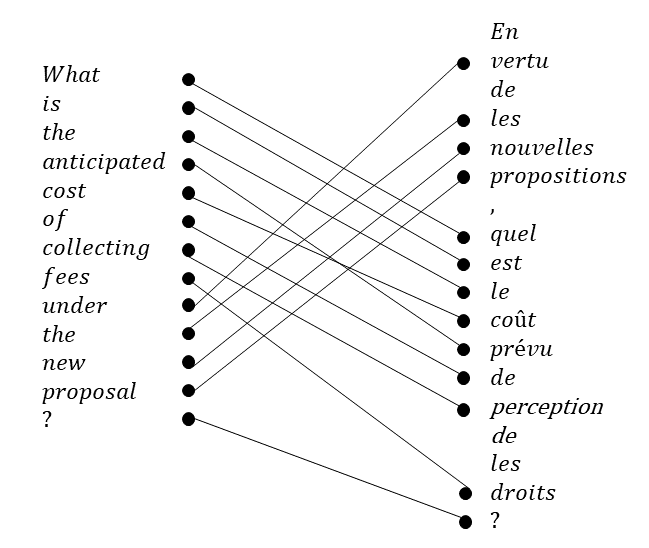
\includegraphics[scale=0.6]{img/lecture_1_word_alignment.png}

Example of word alignments
\end{center}
In this example, if we name $e = e_1, ..., e_E$ the english sentence and $f =
f_1, ..., f_F$ the french one and encode the alignments as $y_{ij} =
\mathbbm{1}(e_i \; linked \; to \; f_j) \in \{0,1\}$ with $(i,j) \in E \times
F$, then we have $|\mathcal{Y}| = 2^{E\times F}$. Adding the constraint
($\sum_i y_{ij} \leq 1$ and $\sum_j y_{ij} \leq 1$) restrains the size of the
output space to $|\mathcal{Y}| = \sum_{k=0}^{\min(E,F)} \begin{pmatrix}
\min(E,F) \\ k \end{pmatrix} \begin{pmatrix} \max(E,F) \\ k \end{pmatrix}$.
\\
\\
More examples of structured prediction problems can be found in Appendix A.
\end{example}

\noindent To specify what is a "\textit{good mapping}", we use a
\textit{structured error} function $l(y, y')$ that assigns a cost to an error
between a prediction $y'$ and the ground truth $y$. We need an error function
on complex labels because not all mistakes are equal.  For instance in machine
translation making a mistake on a single word is not as
bad as getting the whole sentence wrong. In the case of scene labelling it is a
much smaller mistake to label a car as a truck than say, a pedestrian as the
road. Note that error functions do not necessarily have to be \emph{metrics}
as rigorously defined in analysis.
\\
\\
In light of what we introduced, we can characterize structured prediction in
contrast to traditional classification with the following:
\begin{enumerate}
\item The set of labels $\Y$ is usually \textbf{exponential in size}.
\item We need an \textbf{encoding function} to
    represent the labels $y=(y_1,\ldots,y_d)$. The ``pieces'' of $y$ have
    constraints.
\item The prediction task is characterized by a \textbf{structured error/loss
    function} $\ell(y,y')$. In other words we do not automatically get
    an obvious metric for the loss (such as mean squared error in simple
    linear regression).
\end{enumerate}

\section{Structured Prediction Basis and Setup}
Now we will introduce a more formal setting to structured prediction. \\ Given
a training dataset
\begin{equation}
    D \eqbydef (\xi, \yi)_{i=1}^n \qquad \xi \in \X \quad \yi \in \Y \quad i=1,\ldots,n
\end{equation}
we want to learn a \emph{prediction mapping} 
$h_\omega \, : \, \X \rightarrow \Y$ where $\omega$ is a parameter for the
mapping.\\
Moreover we want that mapping to have \emph{low generalization error}:
\begin{equation}
    L(\omega;P) \eqbydef \E_{(x,y) \sim P} [ l(y, h_\omega \given x)]
    \label{eq:vrisk}
\end{equation}
In the above equation, we have:
\begin{itemize}
\item $L$ is the \textit{generalization error}. 
\item $P$ is the \textit{ unknown "test" distribution} on $(x,y)$: $(X, Y) \sim P$.
\item $l: \mathcal{Y}^2 \rightarrow \mathbb{R}$ is the \textit{structured error
    function} which evaluates how bad different prediction mistakes are (not
    all mistakes are equal).
\item $h_w: \mathcal{X} \rightarrow \mathcal{Y}$ is the \textit{predictor}
    parametrized by the random variable $w$ (thus, $L$ is also a random
    variable).
\end{itemize}

\begin{paragraph}
{Note:} It's important to distinguish the \textit{generalization error} (or the
\textit{Vapnik risk} as Simon calls it) from the \textit{frequentist risk}
which is an expectation over all the possible datasets $D$ and \textbf{not} an
expectation over all the possible \textit{ground truth pairs} following $P$ as
it is here. Indeed, if we make the assumptions that all pairs $(x^{(i)},
y^{(i)})$ are i.i.d samples, thus each dataset $D_n$ is a random variable
following a joint distribution $\underbrace{P \otimes.... \otimes P}_{n \;
times}$ noted $P^{\otimes n}$. If we have a \textit{decision procedure} (e.g a
learning algorithm) $A: D_n \mapsto \hat{w_n}$, then the \textit{frequentist
risk} is a summary of the performance of $A$ over all the possible datasets
defined as the following:
\begin{equation}
R_P^F(A) \eqbydef \mathbb{E}_{D_n \sim P^{\otimes n}} \big[L\big(A(D_n);P \big)\big]
\end{equation}
To go deeper, see lectures 4 and 5 of IFT6269 (Probabilistic Graphical Models) for a review of statistical decision theory%
\footnote{\url{http://www.iro.umontreal.ca/~slacoste/teaching/ift6269/A18/}}
\end{paragraph}
\begin{paragraph}
{Note:} In the Machine Learning field, $L$ is simply called "the risk".
\end{paragraph}

\section{Empirical Risk Minimization}
As stated above our goal is to minimize the generalization error, aka the
Vapnik risk as defined in \eqref{eq:vrisk}. However in general we do not have
access to the distribution over which the expectation is taken so that we need
to approximate it. We thus introduce an \textit{empirical version} of this risk
$\hat{L}$ \textit{(the average of the loss function over the training set)}
which has the property to converge for every $w$ towards the target $L$ as the
number of observations $n$ grows. In practice, we will try to minimize with
respect to $w$ a \textit{regularized version of the empirical risk}:
\begin{equation}
    \hat L(\omega) \eqbydef \frac{1}{n}\sum_{i=1}^n l(\yi,h_{\omega}(\xi))
    + R(\omega) \label{eq:erm}
\end{equation} 

The term $R(\omega)$ is a regularizer for the parameter in the above (e.g.
$\vert \vert \cdot \vert \vert ^2$). While we have the information necessary to
compute the above it is rarely easy to miminize; the structured loss functions
(in the summation above) which naturally arise are not convex and/or continuous
in general. While there are techniques to deal with non continuous objective
functions the absence of convexity is a major problem in optimization. 

The solution is to replace the loss function $l$ by a \emph{surrogate loss
function} $\mathcal{L}$ (or a contrast function in the statistics literature).  While there
are many design consideration for such a surrogate loss function the most
commonly required feature is convexity. Examples for such functions
are the structured hinge loss and the log-loss. Yann LeCun 
presents and discusses many of these functions in his paper on energy based
models\footnote{\url{http://yann.lecun.com/exdb/publis/pdf/lecun-06.pdf}}.\\

Substituting those new loss functions into the expression for ERM we 
get the objective function of our optimization problem:
\begin{equation}
    \hat{\mathcal L}(\omega) \eqbydef \frac{1}{n}\sum_{i=1}^n
    \mathcal L (\xi,\yi,\omega)
    + R(\omega) \label{eq:surrogate}
\end{equation}

%The following is copy pasted from 2017 partially latexed scribes by
%Gabriel Huang
\section{Generative vs. Discriminative models.}

Prediction consists in learning a mapping $h_w: \X \longrightarrow \Y$. This
can be done at different levels of modelling and robustness. There is a
tradeoff: a generative model is more powerful --since it explains the data more
completely-- but it is less robust --since it makes more assumptions--, whereas
a simpler, discriminative model explains less but is more robust.
\\
\\
Types of model from least to most discriminative:
\begin{itemize}
\item \textbf{joint-probability $p_w(x,y)$} -- generative model of distribution
    of $x$ and $y$ jointly. The fit to data is the likelihood, and learning is
    done by finding the parameters $w$ maximizing the likelihood (ML). One way
    to make predictions to take $h(x) = \argmax_y p_w(y|x)= \argmax_y
    p_w(x,y)$.
\item \textbf{conditional probability $p_w(y|x)$} --
    conditional generative
    model of the distribution of $y$ once $x$ is fixed. The fit to data is the
    conditional-likelihood, and learning is done by finding the parameters $w$
    maximizing the conditional-likelihood (MCL). One way to make predictions to
    take $h(x) = \argmax_y p_w(y|x)$. 
\item \textbf{prediction mapping
    $y=h_w(x)$} -- discriminative model: instead of a model of $x$ or $y$,
    directly learn a mapping from $x$ to a good label $y$.  The model is
    learned by surrogate loss minimization, which uses information from an
    \textbf{loss function} or \textbf{error function} $l(y,y')$, which in turn
    defines the learning task. 
\end{itemize}

The terminology ``structured prediction" traditionally focuses on prediction
mappings (vs.\ generative modelling), and will be the approach we take in this
course. Loosely speaking, because pointwise estimators are more discriminative,
they are simpler which gives them more power to model more complex labels $y$.
Even though the learned prediction function is not the correct one, we can
still try to find the best one -- in terms of classification error -- among a
class of functions.


\newpage
\begin{appendix}
\chapter{Examples of structured prediction problems}

\begin{example}[optical character recognition]
from an input image $x$ representing a word or sentence, predict the vector $y$
of corresponding letters where each dimension corresponds to successive
letters.  \end{example}

\begin{example}[machine translation]
translate a sentence from one language to the other.

  \centering
    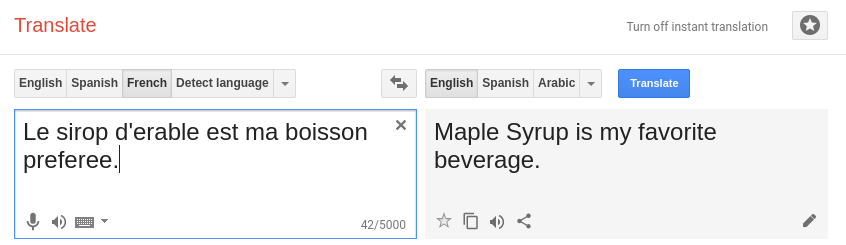
\includegraphics[scale=0.5]{img/googletranslate}
    
Google translate interface.

\end{example}

\begin{example}[3D object recognition]
from a depth map $x$ predict an object map $y$ which maps each pixel location to an object class.
\\

  \centering
    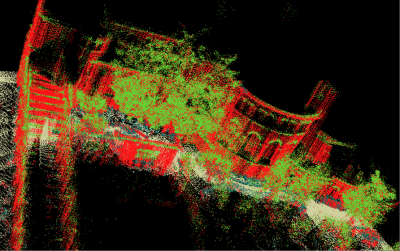
\includegraphics[scale=0.6]{img/3d}
    
Image courtesy of Ben Taskar.
\end{example}

\begin{example}[protein folding]
from a sequence of amino-acids $x$ predict the 3D structure $y$ of the
corresponding protein.

  \centering
    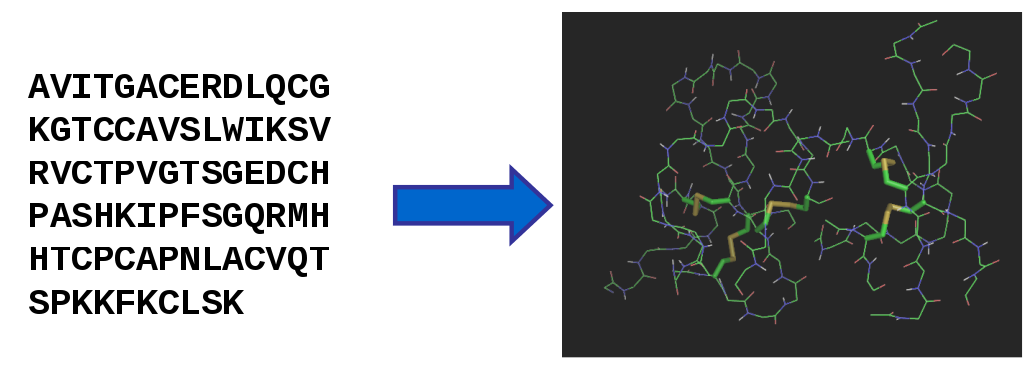
\includegraphics[scale=0.4]{img/proteinfolding}
    
Image courtesy of Ben Taskar.
\end{example}

\begin{example}[text parsing]
from a sentence of words $x$ predict the parse tree(s) $y$ that generated~$x$.

  \centering
    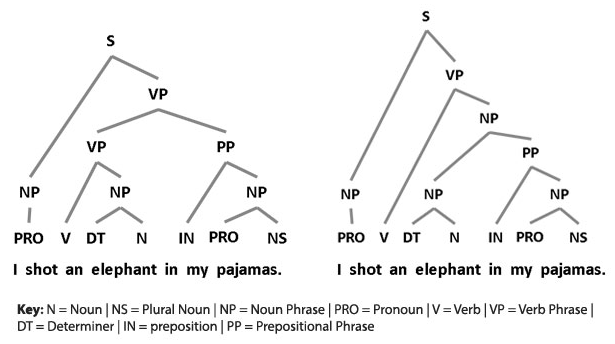
\includegraphics[width=0.5\textwidth]{img/parsetree}
    
Image courtesy of Ron
Daniel%
\footnote{https://www.elsevier.com/connect/new-open-access-resource-will-support-text-mining-and-natural-language-processing}.
\end{example}
\end{appendix}


\end{document}
